%% SECTION HEADER /////////////////////////////////////////////////////////////////////////////////////
\section{Sandwich composite structure}
\label{sec:scs}

%% SECTION CONTENT ////////////////////////////////////////////////////////////////////////////////////
Composites consist of two or more different materials, such as plastics, resins, metal alloys, glass, carbon or bio-based fibres. The combination of material constituents gives  structure benefits from the properties of the component materials, e.g., the strength of carbon fibres and the low density of the polymer resin in the case of \ac{cfrp}.
The contribution of lightweight composite materials to the production of structural components has been increasing rapidly since the middle of the last century.
Composite materials are extensively used in aircraft, aerospace and civil constructions due to their high strength-to-weight ratio, high operating temperatures, great stiffness and high reliability.
For example, composites account for more than 50\% of the total weight of the aircraft Boeing 787 and Airbus A350 \cite{giurgiutiu2015structural}.

One group of composites includes sandwich panels, a multi-layered structure consisting of a mid-core attached between thin shells.
The skins, made of high-strength materials, are designed to carry tensile or compressive stresses from longitudinal forces and bending moments.
On the other hand, the core transmits mainly shear stresses from transverse forces.
It also separates the skins, which increases structural stiffness for thin layers, improves insulation properties, and reduces weight while maintaining strength properties similar to the solid construction of the same density.
A popular core used in engineering structures is a honeycomb geometry core. 
The typical \ac{hsc} is shown in Figure~\ref{fig:hcp}.
The core is composed of lightweight materials, the most common of which include aluminium, cardboard or Nomex\textsuperscript{\tiny\textregistered}.
\begin{figure}[H] %hbtp
	\begin{center}
		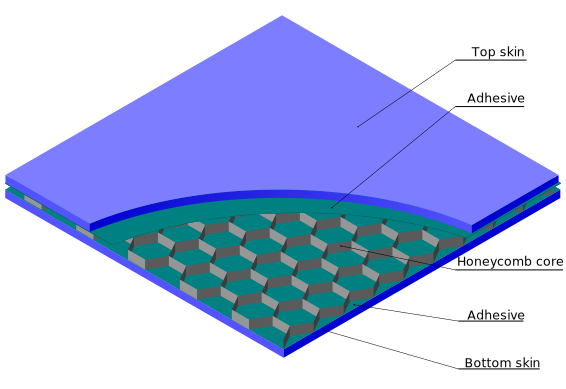
\includegraphics[width=0.95\textwidth]{Intro/honeycomb_plate}
		\caption{
			\label{fig:hcp} Structure of the honeycomb sandwich composite}
		\vspace{-0.5cm}
	\end{center}
\end{figure}

However, various types of damage can occur in these complex structures not found in metal alloy materials. These types of damage include hidden disbonds of the skin and core, delamination of composite skins, or impact damage to the core.
Damage can appear during manufacturing, storage, and operation, so online defect detection methods are required.
Therefore, the increased use of composite materials in the industry has motivated the development of advanced approaches to structural inspections, e.g., methods based on elastic wave propagation had to account for the anisotropic structure of the material.